\documentclass[a4paper,11pt]{ltjsarticle}


% 数式
\usepackage{amsmath,amsfonts,amssymb}
\usepackage{bm}
% 画像
\usepackage{graphicx}

%枠付き文書
\usepackage{ascmac}
\usepackage{fancybox}

\usepackage{listings}
\usepackage{color}

\usepackage{enumitem}
\usepackage{here}

\lstset{
  %プログラム言語(複数の言語に対応,C,C++も可)
  language = Python,
  %背景色と透過度
  backgroundcolor={\color[gray]{.90}},
  %枠外に行った時の自動改行
  breaklines = true,
  %自動改行後のインデント量(デフォルトでは20[pt])
  breakindent = 10pt,
  %標準の書体
  basicstyle = \ttfamily\scriptsize,
  %コメントの書体
  commentstyle = {\itshape \color[cmyk]{1,0.4,1,0}},
  %関数名等の色の設定
  classoffset = 0,
  %キーワード(int, ifなど)の書体
  keywordstyle = {\bfseries \color[cmyk]{0,1,0,0}},
  %表示する文字の書体
  stringstyle = {\ttfamily \color[rgb]{0,0,1}},
  %枠 "t"は上に線を記載, "T"は上に二重線を記載
  %他オプション:leftline,topline,bottomline,lines,single,shadowbox
  frame = TBrl,
  %frameまでの間隔(行番号とプログラムの間)
  framesep = 5pt,
  %行番号の位置
  numbers = left,
  %行番号の間隔
  stepnumber = 1,
  %行番号の書体
  numberstyle = \tiny,
  %タブの大きさ
  tabsize = 4,
  %キャプションの場所("tb"ならば上下両方に記載)
  captionpos = t,
}
\def\lstlistingname{ソースコード}

\begin{document}

\title{CPU実験最終レポート}
\author{7班 05-231001 阿部 桃大}
\date{\today}
\maketitle

\section{7班のコンピュータの構成}
\subsection*{命令セットアーキテクチャ}
命令セットアーキテクチャは、RISC-Vをベースとしている。意図としては、コアにおいて高速実行が可能な回路を構成しやすいようにするためである。

実装した命令は、以下の通りである。

\begin{description}[labelwidth=5em]
  \item[LUI]上位20ビットを即値としてrdに格納
  \item[JAL]即値をpcに加算し、次の命令のアドレスをrdに格納
  \item[JALR]即値をpcに加算し、次の命令のアドレスをrdに格納
  \item[BRANCH]条件分岐命令\\
        \hspace{5em}BEQ, BNE, BLT, BGE, BLTU, BGEU
  \item[LOAD]メモリからデータを読み込む命令\\
        \hspace{5em} LW
  \item[STORE]メモリにデータを書き込む命令\\
        \hspace{5em} SW
  \item[OP-IMM]即値演算命令\\
        \hspace{5em} ADDI,SLLI, SLTI, SLTIU, XORI, SRAI,SRLI,ORI,ANDI
  \item[OP]演算命令\\
        \hspace{5em} ADD, SUB, SLL, SLT, SLTU, XOR, SRA, SRL, OR, AND
  \item[OP\_FP]浮動小数点演算命令\\
        \hspace{5em} FADD,FSUB,FMUL,FDIV,FSQRT,FEQ,FLT,FABS,FCVTWS,FCVTSW
  \item[LOAD\_FP]浮動小数点数を読み込む命令\\
        \hspace{5em} FLW
  \item[STORE\_FP]浮動小数点数を書き込む命令\\
        \hspace{5em} FSW\\
        以降は、独自命令である。
  \item[FADDI]浮動小数点数レジスタを対象に即値を加算する命令
  \item[FLUI]浮動小数点数レジスタを対象に上位20ビットを即値としてrdに格納
  \item[IN/FIN]入力命令
  \item[OUT/FOUT]出力命令
\end{description}

また、コンパイラの出力は、以下の擬似命令も含む。これらの擬似命令は、アセンブラにおいて、上記の命令に変換される。

\begin{description}[labelwidth=3em]
  \item[NOP] 何もしない命令
  \item[LI]即値をrdに格納する命令
  \item[MV]rs1の値をrdに格納する命令
  \item[NOT]rs1のビット反転をrdに格納する命令
  \item[NEG]rs1の符号反転をrdに格納する命令
  \item[SEQZ]rs1==1をrdに格納する命令
  \item[SNEZ]rs1!=1をrdに格納する命令
  \item[SLTZ]rs1<0をrdに格納する命令
  \item[SGTZ]rs1>0をrdに格納する命令
  \item[BEQZ] rs1==0の時分岐する命令
  \item[BNEZ] rs1!=0の時分岐する命令
  \item[BLEZ] rs1<=0の時分岐する命令
  \item[BGEZ] rs1>=0の時分岐する命令
  \item[BLTZ] rs1<0の時分岐する命令
  \item[BGTZ] rs1>0の時分岐する命令
  \item[BLE] rs1<=rs2の時分岐する命令
  \item[BGT] rs1>rs2の時分岐する命令
  \item[BLEU] rs1<=rs2の時分岐する命令(符号無し)
  \item[BGTU] rs1>rs2の時分岐する命令(符号無し)
  \item[J] ラベルにジャンプする命令
  \item[JR] レジスタの値にジャンプする命令
  \item[RET] raの値にジャンプする命令
  \item[CALL] ラベルにジャンプし、次の命令のアドレスをraに格納する命令
  \item[LA] ラベルのアドレスをrdに格納する命令
  \item[FLI] 浮動小数点数の即値をrdに格納する命令
  \item[FMV] 浮動小数点数のrs1の値をrdに格納する命令
\end{description}



\subsection*{コアについて}
コアは、fetch,decode,execute,memory access,write backの5段構成からなるパイプラインプロセッサである。浮動小数演算などのexecuteステージで複数クロックを必要とする命令を実行する際や、メモリアクセスに複数クロック要する場合には、全てのステージにおいてストールが発生する。また、分岐予測は行っておらず、全てuntakenとして予測実行している。

フォアーディングを実装しているため、データハザードによるストールは減らすことに成功している。

レジスタは、通常のRISC-Vの構成である汎用レジスタ32個、浮動小数点レジスタ32個を持っている。

\subsection*{メモリについて}

キャッシュが存在し、以下のような構成になっている。

\begin{description}[labelwidth=5em]
  \item[L1キャッシュ] 16B,1entry
  \item[L2キャッシュ] ダイレクトマップ, 256KB\\\hspace*{4em}
        tagsize: 9bit, indexsize: 14bit, offsetsize: 4bit
\end{description}
L1キャッシュは、最後に書き込みが行われたL2キャッシュのページを保持している。

また、高速化のためにメモリのクロックは、コアのクロックの反転で動いている。

\subsection*{FPUについて}

FPUでは、単精度浮動小数点数を扱う。また、FPUのレジスタは、通常のレジスタとは別になっている。

各命令に対し、以下のクロック数で演算が行われる。

\begin{table}[htb]
  \begin{center}
    \begin{tabular}{|c|c|} \hline
      命令                                 & クロック数 \\ \hline
      FABS,FLT,FGT                       & 2     \\ \hline
      FMUL                               & 3     \\ \hline
      FADD,FSUB,FDIV,FSQRT,FCVTWS,FCVTSW & 5     \\ \hline
    \end{tabular}
  \end{center}
\end{table}


\subsection*{コンパイラについて}

コンパイラは、mincamlをベースにOCamlで実装した。このコンパイラはOCamlのコードを入力として、それを上記の命令セットに変換する。

mincamlで行われる最適化に加えて、以下の最適化を行っている。

\begin{description}[labelwidth=10em]
  \item[レジスタ割り当て] 使わないレジスタを使うように割り当てる。
  \item[スタックの最適化] 積む必要のないスタックを削除する。
  \item[グローバル変数の導入] グローバル変数を絶対アドレスに保持し、それを使うように変換する。
\end{description}

\subsection*{アセンブラについて}
アセンブラは、二つのファイルに分かれている。一つは、アセンブリ言語を機械語に変換するアセンブラであり、もう一つは、機械語をバイナリに変換するアセンブラである。

アセンブリ言語を機械語に変換するアセンブラでは、擬似命令を含む命令列を我々の班の命令セットのみからなる命令列に変換する。

機械語をバイナリに変換するアセンブラでは、機械語をバイナリに変換する。このアセンブラは、機械語をバイナリに変換するだけでなく、機械語のアドレスをラベルに変換する。

\subsection*{シミュレータについて}
シミュレータは、C++で実装した。シミュレーターは、命令列と入力を受け取り、それを実行する。

シミュレータ(ISS)では、以下の実行統計情報を得ることができる。

\begin{description}[labelwidth=10em]
  \item[実行結果] 出力、結果(a0レジスタの値)、各レジスタの値(オプション)
  \item[実行時間予測] 実行命令数、予測実行クロック数、予測実行時間
  \item[メモリ性能]  メモリアクセス回数、キャッシュミス率
  \item[分岐予測] 分岐回数、分岐予測ミス率
  \item[ISSの性能] 実行時間、MIPS
\end{description}

\section{レイトレの実行結果}
レイトレの実行時間は、$256 \times 256$で378.5266sec,$512 \times 512$で1340.1752secであった。また、出力画像は、シミュレータの実行結果と完全に一致し、以下のような画像が出力された。

\begin{figure}[H]
  \begin{center}
    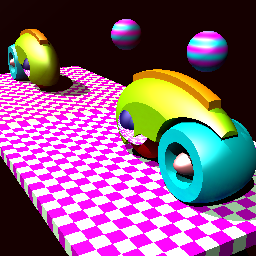
\includegraphics[width=10cm]{out.png}
  \end{center}
  \caption{レイトレの出力画像(256 \times 256)}
\end{figure}

\section{シミュレータについて}
この節では、私の担当であるシミュレータについて説明する。
\subsection*{概要}
全体的な実装の方針として、高速実行できることを重視している。そのため、パイプライン処理は行わず、命令は一つずつ実行するようにしている。

実行時間の正確なシミュレート及び実機でのパラメータ調整を行うため、メモリアクセスと分岐予測の性能を計測している。

シミュレータの実行過程は、以下のようになっている。

\begin{enumerate}
  \item 命令列を構造体に読み込む
  \item 現在のPCに応じた命令を実行し、レジスタやメモリを更新する
  \item 各統計情報、PCを更新し、2に戻る
  \item 命令列の終端に到達したら、終了する
  \item 終了時に統計情報を出力する
\end{enumerate}

\subsection*{ファイル分割}
シミュレータは、以下のようにファイルを分割している。

\begin{description}[labelwidth=7em]
  \item[iss.cpp] シミュレータ本体
  \item[cal.h/cpp] FPU演算の実装
  \item[hardware.h/cpp] pc,クロック,メモリ,レジスタ,分岐予測器などのハードウェア関連の実装
  \item[order.h/cpp] 命令,オペコード,レジスタ名の管理
  \item[print.h/cpp] エラー出力、実行列の出力
\end{description}

なお、iss.cpp以外の各ファイルは、ライブラリとして扱い、アセンブラの実装でも使用している。

\subsection*{FPU演算の実装}
FPU演算はナイーブに実装すると、実機での実行結果から誤差が生じてしまう。そのため、FPU演算は、実機でのverilog実装と全く同じロジックの関数を実装することで、実機での実行結果と一致するようにしている。

また、この実装による出力結果と、デフォルトの単浮動小数演算計算の計算結果を何億ケースも比較し、我々のFPU実装の誤差が要件を満たしていることを確認している。

\subsection*{メモリアクセスの計測}
メモリアクセスに関しては、キャッシュの挙動を正確にシミュレートするようにしている。すなわち、メモリアクセス関数が呼ばれるたびに、キャッシュを参照し、状態に応じて更新およびキャッシュミスのカウントを行っている。

また、シミュレーター上ではL2キャッシュはセットアソシアティブ方式で実装している。実機の実装であるダイレクトマップ方式は、セットアソシアティブ方式の1wayの特殊な場合であるため、シミュレーションは問題なく行える。

シミュレーター上でtag size, index size, offset size,waysを変更することで、最適なキャッシュの構成を探索することができる。上に述べた実機のメモリ構成は、このシミュレーターを用いて探索した結果である。

\subsection*{分岐予測の計測}
最適化の途中で分岐予測器の実装を試していたので、分岐予測器の挙動をシミュレートできるようにしている。

分岐予測器はGshare方式を実装している。Gshare方式は、分岐履歴をPCの値とXORして、その結果をインデックスとして使って飽和カウンタを参照する方式である。

実機での実装においてクリティカルパスが長くなってしまい、実行時間が遅くなってしまうため、最終的には全てuntakenとして予測実行するようにしている。シミュレータでも同様にした。

\subsection*{ストール、フラッシュの実装}
パイプライン処理を行っていないため、ストールやフラッシュが発生する場合を網羅することで、実機と同様のクロック数遷移をするようにしている。

我々のコアにおいてストールが発生するのは、以下の場合である。

\begin{itemize}
  \item 実行に複数クロックを要する命令(FPU演算)を実行する場合
  \item メモリアクセス(どのキャッシュにヒットするかによってクロック数が変わる)
  \item 分岐予測ミス
  \item lw命令によるデータハザード
  \item jal, jalr命令による分岐
\end{itemize}

以上のケースで、それぞれ無駄になるクロック数分だけクロックを進めることで、実機と同様のクロック数遷移をするようにしている。

\subsection*{工夫点}
シミュレータの実装において行った工夫点は、以下の通りである。

\subsubsection*{オプションの実装}
シミュレータには、以下のオプションを実装している。

\begin{description}[labelwidth=5em]
  \item[-p] 命令列の出力
  \item[-r] レジスタの出力
  \item[-t] ISS実行時間の出力
  \item[-d] デバッグモード
  \item[-rt] レイトレ実行用の形式
\end{description}
こうして必ずしも必要でない情報を出力しないことで、実行時間を短縮している。

\subsubsection*{1命令実行あたりの処理の削減}
繰り返し実行されることになる部分を重点的に最適化した。

\begin{itemize}
  \item 命令列は先に構造体に読み込むことで、デコードの時間を削減
  \item シフト演算で書ける部分は、シフト演算を利用
  \item パイプライン処理なしでクロック数シミュレートを行うことで、処理を削減
\end{itemize}

\subsubsection*{最適化オプション}
実行結果が変わらない範囲で、最適化オプションを用いている。makefileには、-Wall -O3 -std=c++17を指定している。

\subsubsection*{パラメータの調整}
パラメータ調整をしやすくするために、各パラメータはヘッダファイルでdefineなどで定義し、一括で変更できるようにしている。

\subsubsection*{実行方法の整備}
実際にテストを行う際には、アセンブリ言語から実行を行いたいことが多い。そのため、Makefileを整備し、アセンブラ、シミュレータを一括で実行できるようにしている。

他にも、コンパイラ係のデバッグにおいては特にコンパイラの出力をシミュレータに入力することが多いため、コンパイラ、アセンブラ、シミュレータの実行を一括で行えるようにシェルスクリプトを整備している。

\subsection*{実行結果}
シミュレータの実行結果は、以下の通りである。

\begin{verbatim}
  simulator result:
  result:         256
  order count: 16139132855
  clocks: 29417656707
  estimated time: 367.721[s] (6m7s)
  memory performance:
  memory access:  6187964979
  l1 cache miss:  4299008145
  l1 cache miss rate:     69.4737[%]
  cache miss:     6757621
  cache miss rate:    0.109206[%]

  branch performance:
  branch count:   766831548
  predict fail:   336853007
  fail rate:     43.9279[%]


  simulator performance:
  simulating time:      120.29[s]
  MIPS:     134.168
\end{verbatim}

予測実行時間は367.721[s]であり、実機での実行時間378.5266[s]との誤差は3\%以内である。

\section{改善点}
最後に、我々の実装において改善点として考えられることを述べる。
\subsection*{全体}
他の班と比較して、我々の班の実行は時間がかかっていた。主な要因となっていたのは、まず命令数の多さである。これは、コンパイラにまだまだ最適化の余地があることを示している。特に、メモリアクセスが161億命令のうちの62億命令を占めていることから、メモリアクセスの最適化が求められる。私はコンパイラについてそこまで詳しくないので、詳しいことはわからないが、ラベル呼び出しの際のレジスタ退避などが無駄になっている可能性がある。また、jal命令やjalr命令を多用しているため、ストールが多く発生していることも要因の一つである。

また、命令セットやコアの構造を最適化しきれていない部分もあった。例えば、レジスタを増やすことで、レジスタ退避を減らすことができるかもしれない。他にも、分岐予測器がないこと、データハザード以外の様々なケースでストールが発生してしまうなど、コアの構造においても改善の余地がある。
\subsection*{シミュレータ}
シミュレータについては主に2つ改善点がある。

まず、実行時間予測が実機との誤差が3\%以内であるが、それでも誤差がある。原因としては、ストールやフラッシュが起こる場合として網羅できていないことが考えられる。様々なケースでテストを行いストールやフラッシュが発生する条件を網羅することで、実機との誤差をさらに減らすことができる。

また、統計データをとらないことでもっと高速に実行できるようにすることも考えられる。現在のシミュレータでは、メモリアクセス、分岐予測の統計データは必ず取るようになっており、処理が増える原因となっている。これらの実装を行う前は現在より$3\thicksim5$倍程度高速であったため、こういった統計データをとらないコードも別に用意すると、そのくらい高速に動作することが期待でき、コンパイラ係のデバッグに役に立つと思われる。

\end{document}
